\documentclass[12pt]{article}

\usepackage{amsmath}
\usepackage{amssymb}
\usepackage{enumitem}
\usepackage{sectsty}
\usepackage[margin=1in]{geometry}
\usepackage{listings}
\usepackage{graphicx}
\usepackage{hyperref}
\usepackage{mdframed}

\hypersetup{colorlinks=true, urlcolor=blue}
\def\UrlBreaks{\do\/\do-}

\sectionfont{\fontsize{14}{15}\selectfont}
\subsectionfont{\fontsize{12}{15}\selectfont}
\lstset{basicstyle=\scriptsize, language=python, frame=single}
\graphicspath{{Handin5/figs/}}

\newcommand{\ddx}[2]{\frac{\mathrm{d}#1}{\mathrm{d}x}#2}
\newcommand{\ppx}[2]{\frac{\partial#1}{\partial#2}}
\newcommand{\supn}[1]{\left|\left|#1\right|\right|_\infty\!}
\newcommand{\dd}{\mathrm{d}}
\newcommand{\intd}[4]{\int_{#1}^{#2}#3\,\mathrm{d}#4\,}
\newcommand{\ltwo}[1]{\left|\left|#1\right|\right|_2\!}
\newcommand{\ltwos}[1]{\left|\left|#1\right|\right|_2^2\!}
\DeclareMathOperator{\sign}{sign}


\begin{document}


\begin{center}
\LARGE{Assignment: Gradient Descent Exploration}
\end{center}


\section*{Part 1: Background}
\begin{enumerate}
\item[(a)]
	Complete weeks one and two of the Coursera Machine Learning course (all the gradient descent stuff).


\item[(b)]
	Read about gradient descent with momentum, as well as RMSProp and Adam.  A good starting point is the wiki page:\\
	\url{https://en.wikipedia.org/wiki/Stochastic_gradient_descent#Extensions_and_variants}\\
	More details can be found here (these are quite a bit more in-depth):\\
	\url{https://blog.paperspace.com/intro-to-optimization-momentum-rmsprop-adam/}
	\url{http://ruder.io/optimizing-gradient-descent/}
\\\\
\end{enumerate}





\section*{Part 2: Introducing the Problem}
Our goal today is to use the variants of gradient descent that you learned about in part 1 to find the $n$-dimensional vector $\mathbf{x}$ that minimizes
$$
	f(\mathbf{x}) = 2 - e^{-r^2} - e^{-100r^2}
$$
where $r^2 = \mathbf{x}\cdot\mathbf{x} / n = (x_1^2 + x_2^2 + ... + x_n^2) / n$.  Clearly the minimum is $f(\mathbf{0}) = 0$.  Our function is symmetric in all dimensions for simplicity, and in one-dimension it looks like this:
\begin{center}
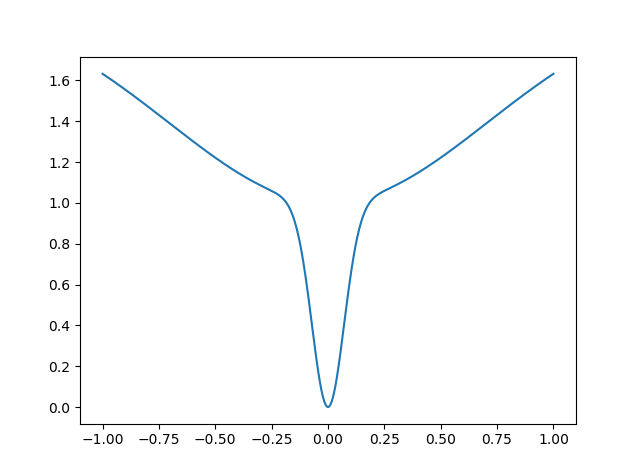
\includegraphics[width=0.75\linewidth]{fx}
\end{center}
This is a convex function, so gradient descent is guaranteed to work, but that sudden change in slope in the middle of the graph is going to cause serious problems for the usual algorithm.  If the learning rate is too small, it will take forever, but if you increase it, it will bounce around inside the well and never find the minimum.  We're going to see how making small changes to the gradient descent algorithm can fix that.\\

\noindent For this problem, we're going to work in 100-dimensions to make things a bit more interesting.  You may think that 100 dimensions is a bit extreme, but note that when training neural networks, we often run gradient descent on millions or tens of millions of dimensions.  Your computer should have no problem working with 100 dimensions, but you can start smaller if you have computational issues or if you get stuck.  The starter code provided includes functions to compute $f$ as well as $\nabla f$:
$$
	\nabla f = 2r^2 \left(e^{-r^2} + 100e^{-100r^2}\right)\mathbf{x}
$$





\section*{Part 3: Solving the Problem}

\begin{enumerate}
\item[(a)]
	Implement the vanilla gradient descent algorithm and try to find the minimum of $f$.  What happens?  A good starting learning rate is 0.01, but you can mess around and see what happens if you change it.
	
	
\item[(b)]
	Implement gradient descent with momentum.  This should only require changing a few lines of your code from part (a) and should make a massive improvement.  Setting the momentum parameter to 0.9 should work fine, and the learning rate can be the same as part (a) or maybe a little higher.  Our algorithm now has a kind of memory of its past trajectory and should be able to find a better minimum, but it's still pretty slow.  It's also less likely to get stuck in weak local minima, which aren't a problem in this case but come up frequently elsewhere.
	

\item[(c)]
	Implement RMSProp.  Again, this should only be a minor change from what you had before.  Keep the decay parameter at 0.9, but decrease the learning rate to 0.001.  Normalizing via the square of the gradient does two things for us.  Firstly, it means that each parameter in $\mathbf{x}$ now gets its own learning rate.  Secondly, it naturally increases and decreases the learning rate for us depending on the structure of the space so we don't have to worry as much about fine-tuning it.  It helps bounce us out of locally flat areas and settle into steeper wells.
	
	
\item[(d)]
	Implement Adam.  Once again, this should not be a substantial change in your code.  Set $\beta_1 = 0.9$, $\beta_2 = 0.99$, and the learning rate to 0.001.  Adam is essentially RMSProp plus momentum and it behaves like a ball rolling under friction.  It avoids flat areas pretty well and settles into steep minima very quickly.  This algorithm is often the go-to for training neural networks, so it's a good one to understand.  Why is it useful to use the normalized $\hat{m}$ and $\hat{v}$ instead of just $m$ and $v$?
		
		
\item[(d)]
	Run each of these algorithms for 50,000 steps starting from \texttt{INIT\_X}.  Plot the value of each algorithm at each step and compare how long it takes for them to converge.  (You probably want a logarithmic plot.  Use \texttt{matplotlib.pyplot.semilogy} or take the log of your algorithm's output at each step.)
	
	
\item[(e)]
	Bonus: Swap the problem down to 2 dimensions and make a fun animation of the convergence of each of these algorithms starting at \texttt{INIT\_X = [-0.7, 0.5]}.  A tutorial for doing so can be found here:\\
	\url{http://louistiao.me/notes/visualizing-and-animating-optimization-algorithms-with-matplotlib/}\\
	This is a decent amount of work, so don't worry too much about it if you don't want to.
\end{enumerate}
\end{document}